\begin{table*}[h]\centering
\begin{tabular}{|l|c|c|c|c|c|}
\hline
                            & PQL2 & PQL3 & PQL+ & WQSP & CWQ \\
\hline
KV-MemNN \cite{DBLP:conf/emnlp/MillerFDKBW16}    & 72.2 & 67.4 & -    & 46.7 / - & 21.1\footnote{The original paper only reports scores on development set.} / -      \\
IRN \cite{DBLP:conf/coling/ZhouHZ18}                         & 72.5 & 71.0   & 52.9 & -    & -         \\
HR-BiLSTM \cite{DBLP:conf/acl/YuYHSXZ17}                  & 97.5 & 87.9 & 92.9 & 62.9 / 62.3 & 33.3 / 31.2         \\
ABWIM \cite{DBLP:journals/corr/abs-1801-09893}                      & 94.3 & 89.3 & 92.6 & -    & -         \\
UHop\footnote{We use the best reported setup from the original paper, aka. ABWIM with UHop.} \cite{DBLP:conf/naacl/ChenCCNK19}                       & 97.5 & 89.3 & 92.3 & -    & -         \\
GRAFT-Net \cite{DBLP:conf/emnlp/SunDZMSC18}                  & -    & -    & -    & 67.8 / 62.5 & 30.1 / 26.0      \\
KBQA with Topic Units \cite{DBLP:conf/ijcai/LanW019}                  & -    & -    & -    & 68.2 / 67.9 & 39.3 / 36.5      \\
\hline
Our Method-obj1             & 98.3 & 97.1 & 97.5 &    62.8 / 62.3  &           \\
Our Method-obj2             &   -   &   -   &   -   &  65.4 / 65.1     &           \\
Our Method-obj3             &     - &  -    &   -   &   67.9 / 67.0    &           \\
Our Method-obj3+new\_decode & -     &   -   &    -   &     &          \\
\hline
\end{tabular}
\caption{\fontsize{10}{12}\selectfont We report Accuracy on PQL and hits@1 and F1 on WQSP and CWQ. All scores except our method are copied from the previous published papers. obj1/2: $P(ans, path|x)= P(ans|path,x)*P(path|x)$ with single/multiple reasoning paths for one sample. obj3: $P(ans) = sum_path(P(ans|path,x)*P(path|x))$, new\_decode: use beam search and multi paths in decoding.}\label{tab:main}
\end{table*}


\begin{figure}[h]
\centering
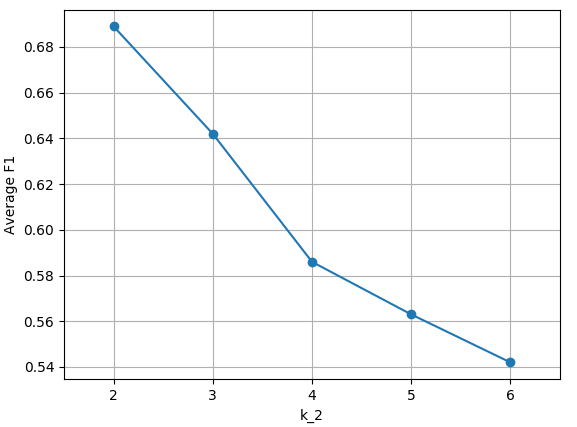
\includegraphics[width=0.85\columnwidth]{figs/fig2.png}
\vspace{-2ex}
\caption{\fontsize{10}{12}\selectfont Average F1 over different thresholds on \textsc{WebQuestionSp} dataset.}
\label{fig:k2}
\end{figure}


\begin{table}[h]\centering
\resizebox{1.01\columnwidth}{!}{
\begin{tabular}{|l|c|c|}
\hline
                           & WQSP & CWQ \\
\hline
%KV-MemNN \cite{DBLP:conf/emnlp/MillerFDKBW16}    & 46.7 / - & 21.1\tablefootnote{The original paper only reports scores on development set.} / -      \\
HR-BiLSTM \cite{DBLP:conf/acl/YuYHSXZ17}                  & 62.9 / 62.3 & 33.3 / 31.2         \\
GRAFT-Net \cite{DBLP:conf/emnlp/SunDZMSC18}                & 67.8 / 62.5 & 30.1 / 26.0      \\
KBQA-GST \cite{DBLP:conf/ijcai/LanW019}          & 68.2 / 67.9 & 39.3 / \textbf{36.5}      \\
\hline
Our Method-joint\_prob             &    62.8 / 62.3  &   36.7 / 31.4        \\
Our Method-joint\_prob\_multiple\_paths             &  65.4 / 65.1     &    - / -       \\
Our Method-marginal\_prob\_with\_true\_label             &   \textbf{68.9} / \textbf{68.5}    &      \textbf{39.4} / 34.8     \\
Our Method-marginal\_prob\_without\_true\_label             &   68.8 / 68.3    &       33.0 / 27.6    \\
%Our Method-obj3+new\_decode  &     &          \\
\hline
\end{tabular}
}
\caption{\fontsize{10}{12}\selectfont We report hits@1 / F1 on WQSP and CWQ.}\label{tab:wqsp_cwq}
\end{table}


A general neural network solution to KBQA is to encode the candidates of relation path or answer into embeddings, and choose or rank these embeddings based on different ranking functions. Existing approaches can be categorized into three types. One is to match the question to a candidate directly via calculating the similarity between them \cite{DBLP:journals/corr/abs-1801-09893,DBLP:conf/adbis/YuHYZW18}. This method is not very suitable for multi-hop questions with long paths, because the number of candidate entity-relation combinations grows exponentially as the number of hops increases. The second type of algorithms is to encode the reasoning information hop by hop, and predict the final answer at the last hop \cite{DBLP:conf/emnlp/MillerFDKBW16,DBLP:conf/coling/ZhouHZ18}, which is a group of methods that are more capable of handling multi-hop questions. Most of these algorithms, however, are restricted to a fixed maximum number of hops, and this number is normally chosen as a relative small number. Recently, a new unrestricted-hop framework is proposed to dynamically choose the number of hops to be executed, by introducing a ``stop'' action to decide when is the last hop \cite{DBLP:conf/naacl/ChenCCNK19}. The third type is specifically designed for multi-hop KBQA, which decompose the input question into several single-hop question, and use the exiting method to solve each simple question. The decomposition methods are based on semantic parsing \cite{DBLP:conf/www/AbujabalYRW17,DBLP:conf/emnlp/LuoLLZ18}, pointer network \cite{DBLP:conf/acl/MinZZH19}, or predefined templates \cite{DBLP:journals/pvldb/ZhengYZC18,DBLP:journals/corr/abs-1807-09623}.  %This number is normally chosen as a relative small number like 1 (single hop), 2 or 3. One main reason is because that, despite theoretically it is possible to search all the possible relations greedily and find the paths starting from the focus entity in the question to the answer entity, the number of all possible entity-relation combinations grows exponentially. It is unrealistic to store or even enlist all these paths when the number of hops is too large. Moreover, it is also unlikely for the system to know the number of hops in advance in real applications. 
 To further improve a multi-hop KBQA system's performance, some recent work also replaces the standard entity linking module by leveraging an augmented topic entity candidate pool \cite{DBLP:conf/ijcai/LanW019}, such that it can cover more entity possibilities. This work is similar to our idea that making use of multiple input information to train the model, but their focus is on entities while ours is on relation paths.
%\kechen{add relation prediction references and multiple relation path, recent ijcai paper?}



\kechen{should we move this to RW? Most of the existing multi-hop KBQA systems \cite{DBLP:conf/acl/YuYHSXZ17,DBLP:journals/corr/abs-1801-09893,DBLP:conf/coling/ZhouHZ18,DBLP:conf/naacl/ChenCCNK19} approach this task by decomposing it into two sub-tasks:
%Currently, there are mainly two main categories of methods to tackle the complex KBQA problems, the first category is based on semantic parsing, and the other category mainly relies on the embeddings (XXX) for information retrieval (IR). %Their differences will be discussed further in the relation work section, and i
%In this paper, we focus on the second category, \emph{i.e.} the embedding based approach, which can either predict the answer directly (XXX) or search (a) relation path(s) leading to the final answer entity (XXX). Conventionally, the relation path searching algorithm consists two main subtasks
topic/focus--entity linking and relation extraction. The topic--entity linking gives the system an entry point to start searching, and the relation extraction is used to search relation paths leading to the final answer. %Unlike the simple single relation questions, for complex questions, the path to the final answer may contains multiple hops, where one hop is defined as a searching step between one entity to another via a single relation. 
For entity linking, there exists many off-the-shell tools  \cite{DBLP:journals/corr/YangC16a} that can give decent performance, and most of the current KBQA models rely on them. For relation extraction, traditional approaches consider all the paths as candidates and search for the best one among them using ranking algorithms.}


We also implement a baseline version of our method with only the question encoding and relation prediction modules. By removing entity lookup and answer prediction modules, our model works similarly as a vanilla RNN model with attention. The baseline model generates a sequence of relations and uses them to fetch the final answer from the knowledge base by following them sequentially. By comparing the last two rows in Table \ref{tab:qpl}, we can see that, by adding the entity lookup module, there is a significant performance boost. It equips our model with the ability not only to search but also to interact with the knowledge base. It can be further observed for Table \ref{tab:qpl} that our model performs much better than the conventional KV-MemNN, which has an entity lookup module, but does not contain a relation prediction module. We believe that this is because the intermediate key-value operations benefit from the direct relation supervision. Therefore, our model can be treated as a good combination of RNN-attention model and KV-MemNN. 


\subsubsection{WebQuestionSP \& ComplexWebQuestion-1.1}
\kechen{only report marginal prob in table 2 and move others to table 3}

\textsc{WebQuestionSP} is a dataset that has been widely used for relation extraction and end-to-end KBQA task. It contains 1 or 2 hops questions with ground truth relation path labels. Table \ref{tab:wqsp_cwq} shows that our model with marginal training objective performs much better than all other methods. KBQA-GST \cite{DBLP:conf/ijcai/LanW019} relies on additional annotations, such as textual description of the knowledge base, and using existing models to generate features. The experiments from their papers show that these generated extra features play a very important role in the system, and their F1 score drops from 67.9 to 61.5 by removing the semantic feature. Similarly, HR-BiLSTM requires relation path annotations to train their model, which are not accessible in many KBQA application scenarios. In contrast, our model supports a training method that takes only raw QA pairs as its input and does not rely on any additional labels or linguistic features. By comparing performance of using different objectives as shown in the second block of the table, we can see that there is a significant improvement by considering multiple relation paths in training. The performance gap between joint objective and marginal objective demonstrates that our proposed marginal objective is a much better way to train a model with multiple relation paths. We do not observe a very different results by using or not using labeled relation paths, which is a good signal. 
Previous stateof-the-art method NSM is only tested on a single dataset. It is unclear whether they could perform consistently well on different datasets. Our full model is shown to consistently work well on three datasets.

\begin{table}[h]\centering
\resizebox{1.01\columnwidth}{!}{
\begin{tabular}{|l|c|c|}
\hline
                           & WQSP & CWQ \\
\hline
KV-MemNN* \cite{DBLP:conf/emnlp/MillerFDKBW16}    &  38.6 &  -      \\
STAGG\_answer* \cite{DBLP:conf/acl/YihRMCS16}  &  66.8 &  -      \\
NSM* \cite{DBLP:conf/acl/LiangBLFL17}  &  69.0 &  -      \\
GRAFT-Net* \cite{DBLP:conf/emnlp/SunDZMSC18}                &  62.8 &  26.0      \\
\hline
STAGG\_SP \cite{DBLP:conf/acl/YihRMCS16}  &  \textbf{71.7} &  -      \\
HR-BiLSTM \cite{DBLP:conf/acl/YuYHSXZ17}                  & 62.3 & 31.2         \\
KBQA-GST \cite{DBLP:conf/ijcai/LanW019}          &  67.9 &  36.5      \\
\hline
Our Method-joint\_prob             &     62.1  &   38.0        \\
Our Method-joint\_prob\_short             &     58.4  &           \\
Our Method-joint\_prob\_random             &     58.8  &           \\
Our Method-joint\_prob\_multiple\_paths             &  63.9     &     -       \\
%Our Method-marginal\_prob\_with\_true\_label             &    \textbf{68.5}    &       34.8     \\
Our Method-marginal\_prob*             &   67.8    &      \textbf{38.4}    \\
%Our Method-obj3+new\_decode  &     &          \\
\hline
\end{tabular}
}
\caption{\fontsize{10}{12}\selectfont We report F1 on WQSP and CWQ. $*$ means this method only requires the final answer as the annotation, and other methods need annotated relation paths or some other annotations.}\label{tab:wqsp_cwq}
\end{table}

\begin{table}[h]\centering
\resizebox{1.01\columnwidth}{!}{
\begin{tabular}{|l|c|c|c|c|}
\hline
                               & \multicolumn{2}{c|}{WQSP}     & \multicolumn{2}{c|}{CWQ}     \\ \hline
                               & 1 path & \textgreater{}1 path & 1 path & \textgreater 1 path \\ \hline
Our Method-joint\_prob         & 60.8   & 63.3                 &    &                \\ 
Our Method-joint\_prob\_short  & 60.0    & 57.0                      &        &                     \\ 
Our Method-joint\_prob\_random &  59.7      &  58.1                    &        &                     \\ 
Our Method-marginal\_prob      & 66.0   & 69.3                 &   &                 \\ \hline
\end{tabular}
}
\caption{\fontsize{10}{12}\selectfont We report F1 on WQSP and CWQ.}\label{tab:wqsp_cwq_path_break}
\end{table}


\begin{table*}[t]\centering
\resizebox{2.1\columnwidth}{!}{%resize the table
\begin{tabular}{l|l|l}
\hline
\multicolumn{3}{c}{Question: what state does romney live in?  \ \ \        Answer: Massachusetts  \ \ \       Topic entity: romney}                                                                                                                                            \\ \hline
.89:children & .29:education\_institution,state\_province\_region & .83:\textbf{places\_lived,location} \\ \hline
.06:\textbf{government\_positions,jurisdiction\_of\_office} & .25:\textbf{places\_lived,location} & .12:\textbf{government\_positions,jurisdiction\_of\_office} \\ \hline
.04:\textbf{government\_positions,office\_position\_or\_title} & .25:\textbf{government\_positions,district\_represented} & .04:\textbf{government\_positions,district\_represented} \\ \hline
.00:\textbf{government\_positions,district\_represented} & .01:\textbf{government\_positions,jurisdiction\_of\_office} & .01:place\_of\_birth,state \\ \hline
.0:place\_of\_birth & .01:place\_of\_birth,state & .00:education,degree \\ \hline
.00:jurisdiction\_of\_office & .01:sibling,place\_of\_birth & .00:election\_campaigns \\ \hline 
\multicolumn{3}{c}{Question:where did madonna grew up?\ \ \       Answer: Bay City\ \ \    Topic entity: madonna}                                                                                                                                            \\ 
\hline
.99:\textbf{place\_of\_birth} & .50:nominated\_for & .47:nominated\_for,featured\_film\_locations \\ \hline
.00:nominated\_for & .16:nominated\_for,featured\_film\_locations & .40:\textbf{place\_of\_birth} \\ \hline
.00:\textbf{place\_lived.location} & .11:compositions & .11:\textbf{place\_lived.location,place} \\ \hline
.00:place\_lived.location,containedby & .09:\textbf{place\_lived.location} & .00:nominated\_for \\ \hline
.00:compositions & .08:\textbf{place\_of\_birth} & .00:\textbf{place\_lived.location} \\ \hline
.00:religion & .01:award\_nominations,nominated\_for & .00:\textbf{place\_lived.location,region} \\ \hline


\end{tabular}
}\caption{\fontsize{10}{12}\selectfont Two running examples from \textsc{WebQuestionSP} dataset. We show the probability $P(\mathbf{r}|q)$ before the inferred relation path. Relation paths that lead to the correct answers are highlighted in bold. The three columns are corresponding to the results by using joint objective with single path, joint objective with multiple paths, and marginal objective with multiple paths. Due to space limit, we only show the partial name of a relation in the example and the probability less than .01 is shown as .00.}\label{tab:case}
\end{table*}

\subsubsection{ComplexWebQuestion-1.1}

This dataset is designed to study complex questions by adding more constraints to questions in \textsc{WebQuestionSP}. It contains more difficult questions than the first two datasets.  We report the experimental results in Table \ref{tab:wqsp_cwq}. Note that this dataset does not come with multiple relation path labels, so the corresponding experiment is not available. Our model outperforms all other models in terms of hits@1, and slightly worse than KBQA-GST in terms of F1 score, but again, KBQA-GST requires many additional information to train. Different from the observation in \textsc{WebQuestionSP} dataset, we see that there is a performance degradation when the model is not pre-trained with ground truth relations. It is because that the model can easily make errors in early stage and gets stuck with these errors. In contrast, our model on WQSP does not suffer from this problem because the relation path is much shorter, and thus it is not hard to generate correct training samples at the beginning of the training. To compare it with existing methods, our model still performs better than GRAFT-Net, which is the state-of-the-art results without using any additional labels.
